\documentclass[runningheads]{llncs}
\usepackage[T1]{fontenc}
\usepackage{lmodern}
\usepackage{graphicx}
\usepackage{amsmath,amssymb}
\usepackage{booktabs}
\usepackage{multirow}
\usepackage{tabularx}
\usepackage[table]{xcolor}
\usepackage{tikz}
\usetikzlibrary{positioning,arrows.meta,fit}
\usepackage{microtype}
\usepackage[hidelinks]{hyperref}
\usepackage{enumitem}
\setlist{nosep,leftmargin=*}

\providecommand{\TBD}{\textcolor{red}{TBD}}
\newcommand{\pending}[1]{\textcolor{red}{[#1]}}
% Generated by paper/make_numbers.py. Do not edit by hand.
\providecommand{\TBD}{\textcolor{red}{TBD}}
\newcommand{\SynSeeds}{7}
\newcommand{\SynRows}{945{,}626}
\newcommand{\SynPairs}{200{,}840}
\newcommand{\SynMalPairs}{4}
\newcommand{\SynDecoyPairs}{2}
\newcommand{\SynRuntime}{44}
\newcommand{\FunPrefilteredChannels}{2{,}351}
\newcommand{\FunAnomFlows}{15{,}640}
\newcommand{\FunSax}{7}
\newcommand{\FunSaxPass}{7}
\newcommand{\FunBeacon}{7}
\newcommand{\FunCorr}{4}
\newcommand{\FunIforestPairs}{7}
\newcommand{\SynCorrP}{1.00}
\newcommand{\SynCorrR}{1.00}
\newcommand{\SynCorrF}{1.00}
\newcommand{\SynBeaconP}{0.65$\pm$0.04}
\newcommand{\SynBeaconR}{1.00}
\newcommand{\SynBeaconF}{0.79$\pm$0.03}
\newcommand{\SynAP}{1.00}
\newcommand{\OldEvalF}{1.00}
\newcommand{\HtwoPairs}{49}
\newcommand{\HtwoTrue}{49}
\newcommand{\DecoyCorrMax}{0.537}
\newcommand{\DecoyCorrMargin}{0.013}
\newcommand{\SynScenRows}{%
\texttt{exfil\_slow} & mal. & 6.00\,h (8\%) & 6.07\,h & 0.96 & 0.67 & corroborated \\
\texttt{fast\_https\_dga} & mal. & 5.0\,min (10\%) & 5.0\,min & 0.95 & 0.57 & corroborated \\
\texttt{multi\_host\_campaign} & mal. & 15.0\,min (15\%) & 15.0\,min & 0.92 & 0.71 & corroborated \\
\texttt{slow\_http\_fixed} & mal. & 1.00\,h (5\%) & 1.00\,h & 0.97 & 0.93 & corroborated \\
\texttt{decoy\_ntp} & decoy & 17.1\,min (5\%) & 17.0\,min & 0.97 & 0.54 & beacon uncorroborated \\
\texttt{decoy\_windows\_update} & decoy & 1.00\,h (20\%) & 59.7\,min & 0.89 & 0.39 & beacon uncorroborated \\}
\newcommand{\SynAblateRows}{%
IForest anomaly (stages 1-4) & 0.65$\pm$0.04 & 1.00 & 2.1$\pm$0.4 \\
+ SAX pass (stage 5) & 0.65$\pm$0.04 & 1.00 & 2.1$\pm$0.4 \\
+ periodicity (stage 6) & 0.65$\pm$0.04 & 1.00 & 2.1$\pm$0.4 \\
+ corroboration (stage 9) & 1.00 & 1.00 & 0.0 \\
\midrule
Spectral term on counts (this paper) & 0.65$\pm$0.04 & 1.00 & F1$_{corr}$ 1.00 \\
Spectral term on IAT index (uninformative) & \multicolumn{3}{c}{pending} \\
No spectral term & \multicolumn{3}{c}{pending} \\}
\newcommand{\ExfilConfFix}{0.96}
\newcommand{\ExfilConfOrig}{\TBD}
\newcommand{\ExfilConfNone}{\TBD}
\newcommand{\RealRows}{%
\multicolumn{9}{c}{\textit{Real-data runs pending}} \\}
\newcommand{\RealPeriodRows}{%
\multicolumn{5}{c}{\textit{pending}} \\}
\newcommand{\RealRuns}{0}


\begin{document}

\title{CADENCE: C2 Anomaly Detection via Ensemble Network Correlation Evidence}
\titlerunning{CADENCE: C2 Beacon Detection on Zeek Telemetry}
\author{Jack D. Moody}
\authorrunning{J. D. Moody}
\institute{Whiting School of Engineering, Johns Hopkins University, Baltimore, MD, USA\\
\email{jmoody11@jhu.edu}}

\maketitle

\begin{abstract}
Command-and-control (C2) beaconing is rarely visible in any single connection. It is visible in behavior over time: regular callbacks to one destination, uniform payloads, and correlated traces across protocol layers. We present CADENCE, an unsupervised ten-stage pipeline over Zeek logs that reduces hundreds of thousands of connections to a handful of analyst-ready leads. The stages are domain-knowledge pre-filtering, Isolation Forest scoring of fourteen channel features, symbolic (SAX) pre-screening, periodicity estimation from the autocorrelation and Welch spectrum of a binned connection-count series, PELT changepoint detection, six-hypothesis DNS/HTTP/TLS corroboration with adaptive weighting, and MITRE ATT\&CK annotation. We score detection per source--destination pair and attribute every missed C2 pair to the stage that dropped it. On 30-day synthetic telemetry (\SynRows{} connections, \SynSeeds{} seeds) CADENCE recovers all \SynMalPairs{} malicious beacons with no false positives. Two periodic decoys pass every timing test and are removed only by corroboration, but by a fixed margin of \DecoyCorrMargin{} below the lead threshold rather than by contrary evidence. \pending{Real-data headline: CTU-13 scenarios and lab captures of current C2 frameworks, filled from results/real\_data.} We also document an evaluation pitfall: a Welch spectrum computed over the inter-arrival \emph{index} sequence, rather than a time-sampled series, is uninformative, and we give the corrected construction.
\keywords{C2 beaconing \and Network anomaly detection \and Periodicity analysis \and Zeek \and Threat hunting \and Evaluation methodology}
\end{abstract}

%=====================================================================
\section{Introduction}
%=====================================================================

Advanced persistent threat (APT) operators keep access to compromised networks through command-and-control (C2) channels. An implant calls back on a schedule to fetch tasking, report results, and stage data. One callback looks like ordinary traffic: a few hundred bytes to a plausible host on port 443. What gives it away is its behavior over weeks. It fires at a near-constant interval, to the same destination, with stereotyped payloads, and it leaves matching traces in DNS, HTTP, and TLS logs.

Enterprise sensors produce hundreds of thousands of Zeek~\cite{paxson1999bro} \texttt{conn.log} records per day. Threat hunters cannot read them, so triage must shrink the candidate set to a few high-confidence leads without losing real beacons. CADENCE is built around one idea. Each stage answers a single question the previous stage cannot, and each stage hands a smaller, cleaner set to a more expensive test.

Beacon detectors are often evaluated on traffic their authors generated, with metrics computed at whatever unit is most convenient. Both choices inflate results~\cite{sommer2010closed,arp2022dos}. We therefore pair the system with an evaluation protocol that is strict about the unit of detection and transparent about failure. This paper makes four contributions:
\begin{itemize}
\item \textbf{CADENCE}, a staged, unsupervised C2 beacon detector over Zeek logs. It combines channel-level anomaly scoring, symbolic pre-screening, jitter-tolerant periodicity estimation, changepoint timing, adaptive DNS/HTTP/TLS corroboration, and ATT\&CK annotation (Sect.~\ref{sec:method}).
\item \textbf{A pair-level evaluation protocol} with stage attribution of misses, strict and lenient treatment of non-C2 malicious traffic, and tooling that runs the pipeline on public pcap and Zeek datasets (Sect.~\ref{sec:setup}).
\item \textbf{Results} on synthetic telemetry across \SynSeeds{} seeds and on public real traffic. The real traffic covers CTU-13 botnet captures~\cite{garcia2014ctu13} and lab captures of current C2 frameworks with published beacon parameters~\cite{acm_motd} (Sect.~\ref{sec:results}).
\item \textbf{Two evaluation findings} that change how such pipelines should be read. First, a common spectral-confirmation shortcut is uninformative; we give the corrected construction and an ablation (Sect.~\ref{sec:spectral}). Second, host-scoped DNS evidence makes decoy suppression rest on a threshold margin rather than on discriminating evidence (Sect.~\ref{sec:discussion}).
\end{itemize}

%=====================================================================
\section{Related Work}
%=====================================================================

\paragraph{Periodicity-based beacon detection.}
BotFinder learns per-family models of C2 trace features, including the regularity of flow inter-arrival times, from NetFlow without payloads~\cite{tegeler2012botfinder}. Disclosure detects C2 servers from large-scale NetFlow using flow-size, client-access, and temporal features~\cite{bilge2012disclosure}. BAYWATCH finds beaconing in five months of enterprise web-proxy logs with signal-processing periodicity detection followed by an eight-step filter that removes legitimate periodic traffic~\cite{hu2016baywatch}. Zhang et al.\ aggregate signals across protocols and networks to recover periodicity hidden by jitter, and rank candidates with self-training and active learning~\cite{zhang2023aggregation}. RITA scores beacons from Zeek logs with interval and size regularity statistics~\cite{rita}. CADENCE shares the premise that periodicity alone over-alarms on benign automation. It differs in the order of operations. Cheap volumetric and symbolic filters run first, periodicity is estimated on a binned count series that tolerates jitter, and the final decision rests on cross-layer evidence rather than on periodicity strength.

\paragraph{Unsupervised anomaly detection and symbolic time series.}
Isolation Forest~\cite{liu2008iforest} scales to large feature tables without density assumptions, unlike one-class SVM~\cite{scholkopf2001ocsvm} and LOF~\cite{breunig2000lof}. SAX~\cite{lin2003sax} discretizes time series for fast pattern tests. CADENCE uses it only as a cheap gate before spectral analysis.

\paragraph{Cross-protocol and DNS evidence.}
BotHunter correlates IDS alerts into infection dialogs~\cite{gu2007bothunter}, and Beehive mines enterprise logs for suspicious hosts~\cite{yen2013beehive}. DNS indicators include algorithmically generated domains~\cite{yadav2010dga,antonakakis2012dga} and fast-flux hosting~\cite{holz2008fastflux}. CADENCE applies such indicators only to pairs that have already shown periodic structure, as tests of a specific hypothesis.

\paragraph{Evaluation practice.}
Sommer and Paxson~\cite{sommer2010closed} and Arp et al.~\cite{arp2022dos} catalogue pitfalls that inflate learning-based security results. These include sampling bias, data snooping, inappropriate baselines, and lab-only evaluation. Our protocol responds to these directly. It scores the unit the detector flags, fixes the configuration before looking at real-data results, and reports where each miss occurs.

%=====================================================================
\section{Problem and Threat Model}
%=====================================================================

The input is a window of Zeek logs: \texttt{conn.log} is required, and \texttt{dns.log}, \texttt{http.log}, and \texttt{ssl.log} are optional. A \emph{pair} $(s,d)$ is an originator and responder address. A \emph{channel} refines a pair by destination port and service. The task is to flag the pairs that carry C2, and to attach to each one the evidence an analyst needs to act. We assume an implant that calls back at a mean interval $T$ with bounded jitter, from an internal host to an external destination, for long enough to produce at least eight connections in the window. We do not address C2 with no periodic connection structure, such as purely interactive sessions or long-lived single connections. We also do not address C2 hidden behind high-fan-in shared infrastructure such as CDN fronting. Both are discussed in Sect.~\ref{sec:discussion}. CADENCE runs offline on retrospective windows, as in hunt operations. It does not perform streaming enforcement.

%=====================================================================
\section{Method}\label{sec:method}
%=====================================================================

Figure~\ref{fig:pipeline} shows the ten stages. Defaults are given in parentheses. All are configuration values, and none was fit to the real-data results reported here.

\begin{figure}[tbp]
\centering
\resizebox{\textwidth}{!}{%
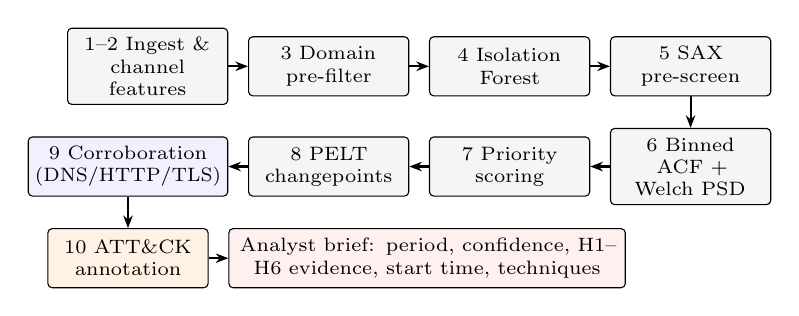
\begin{tikzpicture}[
  node distance=2.0mm and 2.5mm,
  st/.style={draw,rounded corners=1.5pt,minimum height=7.5mm,text width=18mm,align=center,font=\scriptsize,fill=gray!8},
  ev/.style={st,fill=blue!6,text width=23mm},
  ar/.style={-{Stealth[length=1.6mm]},thick}]
\node[st] (a) {1--2 Ingest \&\\channel features};
\node[st,right=of a] (b) {3 Domain\\pre-filter};
\node[st,right=of b] (c) {4 Isolation\\Forest};
\node[st,right=of c] (d) {5 SAX\\pre-screen};
\node[st,below=4mm of d] (e) {6 Binned ACF +\\Welch PSD};
\node[st,left=of e] (f) {7 Priority\\scoring};
\node[st,left=of f] (g) {8 PELT\\changepoints};
\node[ev,left=of g] (h) {9 Corroboration\\(DNS/HTTP/TLS)};
\node[st,below=4mm of h,fill=orange!10] (i) {10 ATT\&CK\\annotation};
\node[st,right=of i,text width=48mm,fill=red!6] (j) {Analyst brief: period, confidence, H1--H6 evidence, start time, techniques};
\draw[ar] (a)--(b); \draw[ar] (b)--(c); \draw[ar] (c)--(d); \draw[ar] (d)--(e);
\draw[ar] (e)--(f); \draw[ar] (f)--(g); \draw[ar] (g)--(h); \draw[ar] (h)--(i); \draw[ar] (i)--(j);
\end{tikzpicture}}
\caption{The CADENCE pipeline. Stages 1--4 work on channels, Stages 5--10 on $(s,d)$ pairs. Each stage passes a smaller set to a more expensive test.}
\label{fig:pipeline}
\end{figure}

\subsection{Stages 1--4: Channels, Pre-filter, Isolation Forest}

Connections are grouped into channels keyed by $(s, d, \text{port}, \text{service})$, and channels with fewer than eight flows are dropped. Each channel is summarized by fourteen features:
\begin{itemize}
\item \emph{volume}: log flow count;
\item \emph{timing}: inter-arrival time (IAT) coefficient of variation, log mean IAT, IAT median absolute deviation, median-to-mean IAT ratio, and missing-beat rate (the fraction of expected slots at the median IAT with no connection);
\item \emph{persistence}: the fraction of days active;
\item \emph{payload}: bytes CV, request/response asymmetry, and zero-payload fraction;
\item \emph{connection consistency}: duration CV and connection-state entropy;
\item \emph{time of day}: mean sine and cosine of the hour.
\end{itemize}
Features are standardized.

The pre-filter removes channels that cannot be C2 under the threat model. These are internal-to-internal channels, where RFC~1918 space is extended by configured internal ranges; destinations that are well-known public DNS resolvers, NTP servers, or CDN prefixes; infrastructure ports on internal destinations; destinations contacted by more than half of all sources (applied only when there are at least ten sources); and channels with at least 90\% failed connection states.

An Isolation Forest~\cite{liu2008iforest} (200 trees, 3{,}000 samples per tree, contamination 0.05) scores the remaining channels. A stability check refits on a 70/30 split and warns if score agreement falls below 0.80. The flows of anomalous channels are then regrouped by $(s,d)$ for the timing stages.

\subsection{Stage 5: Symbolic Pre-screening}

A pair can be volumetrically odd but aperiodic. Its IAT sequence is z-normalized, reduced by piecewise aggregate approximation to $w{=}20$ segments, and mapped to an alphabet of four symbols~\cite{lin2003sax}. Three $O(n)$ tests follow. The first is a symbol CV below 0.60. The second is a peak $|\text{ACF}|$ above 0.30 within ten symbol lags. The third is a repeated-prefix motif that covers more than 40\% of the word. Pairs passing two of the three tests, with at least eight observations, go on to the full periodicity analysis.

\subsection{Stage 6: Periodicity from a Binned Count Series}\label{sec:spectral}

Autocorrelation of raw IATs fails for jittered beacons, because successive intervals are nearly independent draws. CADENCE instead bins connection timestamps with width $\Delta = \tilde{\tau}/2$, where $\tilde{\tau}$ is the median IAT. This gives a count series $c_k$. A beacon with period $T \approx \tilde{\tau}$ places roughly one event in every other bin, so the ACF of $c_k$ peaks at lag~2 even under substantial jitter. The ACF peak $a$ (lags up to 40, significance threshold 0.25) gives the period $T_{\text{acf}} = \ell^\ast \Delta$.

\emph{Spectral confirmation.} We compute a Welch periodogram~\cite{welch1967} of $c_k$ with sampling rate $f_s = 1/\Delta$ (64-sample segments), so frequencies are in hertz and periods in seconds. Over periods of at least $T_{\min}=60$\,s we take the peak frequency, and the share $\rho$ of spectral power that falls in that peak bin. On controlled signals, beacons with up to 30\% uniform jitter give $\rho \in [0.15, 0.67]$ at the correct period, from 5\,min to 6\,h. Poisson, uniform, heavy-tailed, and business-hours traffic give $\rho \in [0.04, 0.06]$.

The construction matters. An earlier version of CADENCE ran Welch on the IAT sequence itself with $f_s = 1$, a natural shortcut. Its ``periods'' are then counted in beacons, not seconds. Against a 60\,s floor, the only admissible bin is the lowest nonzero frequency of a 64-sample segment, so every pair with at least 60 observations returns period 64 and $\rho = 1$ whether it is periodic or not, and pairs with fewer return $\rho=0$. The spectral term then only measures how many observations a pair has. Section~\ref{sec:results} quantifies its effect.

\emph{Confidence.} With IAT coefficient of variation $v$, the beacon confidence is
\begin{equation}
c = 0.4\min\!\left(1,\tfrac{a}{0.25}\right) + 0.3\max\!\left(0, 1-\tfrac{v}{0.60}\right) + 0.2\min\!\left(1,\tfrac{\rho}{0.15}\right) + 0.1\,\mathbb{1}[\text{periodic}],
\end{equation}
where \emph{periodic} requires $v < 0.60$, $T \ge T_{\min}$, and either the ACF or the spectral test to pass. A pair is a beacon if $c \ge 0.45$.

\subsection{Stages 7--8: Priority and Changepoints}

A priority score out of 10 ranks pairs for review. It weights beacon confidence $\times4$, payload stability $\times2$, multi-day persistence $\times2$, agreement between the connection period and the DNS/HTTP cadence $\times1$, and off-hours activity $\times1$. PELT~\cite{killick2012pelt} with an $L_2$ cost, a penalty of $2\sigma^2\log n$, and a minimum segment length of five is applied to each beacon's IAT sequence. It estimates when beaconing began and flags interval changes that suggest operator reconfiguration.

\subsection{Stage 9: Cross-layer Corroboration}

Periodicity cannot separate C2 from update agents or NTP. For each beacon pair, CADENCE tests six hypotheses against the protocol logs:
\begin{itemize}
\item \textbf{H1} DNS regularity: the source resolves a domain whose answers include $d$, at the beacon period (within 15\%), with a minimum count scaled to the expected number of firings.
\item \textbf{H2} DNS anomaly: algorithmically generated labels (entropy above 3.5 bits on labels of at least 8 characters), fast flux, or NXDomain rate above 10\%.
\item \textbf{H3} HTTP consistency: low response-body CV ($<0.30$) and URI-length CV ($<0.40$).
\item \textbf{H4} HTTP evasion: user agents that are rare network-wide, high-entropy URIs, or unusual methods.
\item \textbf{H5} TLS consistency: a stable SNI, a monotonic JA3, and certificate reuse.
\item \textbf{H6} TLS evasion: a self-signed or new certificate, a known C2 JA3, an absent SNI, or a high session-resumption rate.
\end{itemize}
Known-benign services, such as Microsoft update agents and common library user agents, are excluded first. The corroboration score combines continuous DNS, HTTP, and TLS sub-scores with the six hypothesis outcomes, using weights that adapt to which logs exist for the pair (Table~\ref{tab:weights}). The absence of a log type is therefore neutral. Encrypted C2 with no HTTP visibility is judged on DNS and TLS rather than penalized. A pair becomes a lead if $S \ge 0.55$.

\begin{table}[tbp]
\centering\scriptsize
\caption{Adaptive corroboration weights. $B$ is the weighted share of passed hypotheses within the tier.}\label{tab:weights}
\setlength{\tabcolsep}{3pt}
\begin{tabular}{@{}lll@{}}
\toprule
Logs & Score $S$ & Weights within $B$\\
\midrule
HTTP+TLS & $.30S_{\text{dns}}+.30S_{\text{http}}+.20S_{\text{tls}}+.20B$ & H1 .20, H2 .25, H3--4 .15, H5 .13, H6 .12\\
HTTP & $.20S_{\text{dns}}+.20S_{\text{http}}+.60B$ & H1 .25, H2 .35, H3--4 .20\\
TLS & $.40S_{\text{dns}}+.40S_{\text{tls}}+.20B$ & H1 .25, H2 .35, H5--6 .20\\
DNS only & $.45S_{\text{dns}}+.55B$ & H1 .35, H2 .65\\
\bottomrule
\end{tabular}
\end{table}

\subsection{Stage 10: ATT\&CK Annotation}

Each lead is annotated with the ATT\&CK techniques~\cite{strom2018attack} that its evidence supports:
\begin{itemize}
\item T1029 (Scheduled Transfer) from a confirmed period;
\item T1568.002 (DGA) from H2;
\item T1071.001 (Web Protocols) from H3;
\item T1036 (Masquerading) from a rare user agent;
\item T1573 (Encrypted Channel) for periodic pairs with no HTTP visibility;
\item T1132 and T1001 (data encoding and obfuscation) from high-entropy URIs;
\item T1041 (Exfiltration Over C2 Channel) from sustained periodic volume.
\end{itemize}
The analyst brief groups the techniques by tactic, next to the evidence for each.

%=====================================================================
\section{Experimental Setup}\label{sec:setup}
%=====================================================================

\paragraph{Unit and ground truth.} Stages 5--10 flag $(s,d)$ pairs, so we score pairs. A pair is positive if any of its flows carries a C2 label in the source data. Infected-host traffic that is not C2, such as spam or scanning, is labelled \emph{malicious-other}. It is scored two ways: \emph{strict} counts it as negative, and \emph{lenient} drops it from the universe. We report precision, recall, and F1 at two operating points, ``beacon'' (end of Stage~6) and ``lead'' (end of Stage~9). We also report average precision over a ranking that orders pairs by the furthest stage reached and then by the confidence at that stage. Every C2 pair is attributed to the furthest stage it reached, so each miss has a stated cause. The earlier evaluation in this line of work credited a scenario as detected when either endpoint of a lead appeared in that scenario's traffic, and counted false positives per pair. Under that rule a benign lead that shares a host with a beacon still counts as a detection.

\paragraph{Protocol.} All results use the default configuration. Two settings change per dataset, and only for reasons that come from the dataset itself rather than from detection results: the internal address range, and the period floor $T_{\min}$ when a capture's published beacon interval is below 60\,s. Any configuration chosen after seeing results is reported separately as tuned.

\paragraph{Synthetic data.} The generator produces 30 days of enterprise traffic (about 30{,}000 background connections per day plus a noisy host), matching DNS, HTTP, and TLS logs, and six injected scenarios with Gaussian interval jitter (Table~\ref{tab:synth}). Four are malicious. The two decoys, a Windows update agent and NTP polling, are genuinely periodic and pass every timing test, so only corroboration can remove them. We run \SynSeeds{} seeds (42 and 0--9).

\paragraph{Real data.} \emph{CTU-13}~\cite{garcia2014ctu13} contains thirteen captures of real botnets (Neris, Rbot, Virut, Menti, Sogou, Murlo, NSIS.ay) mixed with university background traffic. Every flow carries a manual label, and command-and-control flows are distinguished. We run Zeek on the truncated full-capture pcaps and derive pair labels from the labelled bidirectional NetFlows. The truncated capture retains little application payload for background traffic, while botnet traffic was also captured in full. Corroboration on this data would therefore separate the classes artificially. We report conn-only results as the headline and corroboration only as an ablation. \emph{Active Countermeasures ``Malware of the Day''}~\cite{acm_motd} publishes 24-hour lab captures of current C2 frameworks (e.g., Cobalt Strike, Sliver) with the victim, C2 server, beacon interval, and jitter stated. These give exact ground truth for modern implants. \pending{IoT-23~\cite{parmisano2020iot23} if completed.}

\paragraph{Implementation.} CADENCE is written in Python with scikit-learn~\cite{pedregosa2011sklearn}, SciPy~\cite{virtanen2020scipy}, and statsmodels. An adapter converts native Zeek TSV/JSON logs or pcaps into the pipeline's input. Experiments ran on a 2-vCPU, 7\,GB cloud VM. A 30-day synthetic run (about 945k connections) takes \SynRuntime\,s end to end. Code, configurations, and per-run outputs are public.\footnote{\url{https://github.com/jackdmoody/CADENCE}}

%=====================================================================
\section{Results}\label{sec:results}
%=====================================================================

\subsection{Synthetic Telemetry}

\begin{table}[tbp]
\centering\scriptsize
\caption{Synthetic scenarios (seed 42). Period is true (Gaussian jitter $\sigma$ as \% of period) and estimated. $c$: beacon confidence; $S$: corroboration score (lead if $\ge 0.55$).}\label{tab:synth}
\begin{tabular}{@{}llrrrrl@{}}
\toprule
Scenario & Type & True period & Estimated & $c$ & $S$ & Furthest stage\\
\midrule
\SynScenRows
\bottomrule
\end{tabular}
\end{table}

On seed 42 the window holds \SynRows{} connections between \SynPairs{} pairs. The pre-filter removes \FunPrefilteredChannels{} channels. Isolation Forest passes \FunIforestPairs{} pairs (\FunAnomFlows{} flows), SAX passes \FunSaxPass{}, and periodicity confirms \FunBeacon{}. Corroboration then keeps \FunCorr{} leads. Across \SynSeeds{} seeds the lead stage reaches precision \SynCorrP{}, recall \SynCorrR{}, and F1 \SynCorrF{}. The beacon stage reaches precision \SynBeaconP{} at recall \SynBeaconR{}. Table~\ref{tab:synth} shows why. Both decoys are strongly periodic ($c > 0.9$) and are suppressed only at Stage~9. Period estimates fall within a few percent of the truth, from 5\,min to 6\,h.

The way the decoys are suppressed matters more than the fact that they are. H2 (DNS anomaly) was true for \HtwoTrue{} of the \HtwoPairs{} candidate pairs scored across seeds, including both decoys on every seed. For a pair with no HTTP or TLS records, H2 alone gives $S = 0.45 \cdot 0.40 + 0.55 \cdot 0.65 = 0.5375$. The NTP decoy, and the one non-beacon pair that reached Stage~9, land at exactly that value on every seed, \DecoyCorrMargin{} below the threshold. Decoy suppression on this data is therefore a property of the weights and the threshold, not of evidence that separates the decoys from C2 (Sect.~\ref{sec:discussion}).

\begin{table}[tbp]
\centering\scriptsize
\caption{Ablations over \SynSeeds{} seeds (mean$\pm$sd). Top: alarming on every pair that reaches a stage. Bottom: spectral-term variants.}\label{tab:ablate}
\begin{tabular}{@{}lccc@{}}
\toprule
Configuration & Precision & Recall & False positives\\
\midrule
\SynAblateRows
\bottomrule
\end{tabular}
\end{table}

Table~\ref{tab:ablate} (top) separates the contributions, and it is a warning about synthetic data. Isolation Forest reduces about 200k pairs to \FunIforestPairs{}, and every one of them clears the SAX and periodicity stages. The first three rows are identical. The generator's background is aperiodic by construction, so this data does not exercise the timing stages as filters. Only corroboration removes the two or three non-malicious pairs per seed.

The spectral variants (bottom) show that on this data the spectral term changes nothing that matters. The lead stage is perfect under all three variants. Apart from the noisy host, every pair that reaches Stage~6 is genuinely periodic and has at least 60 observations, so the original construction's constant credit happens to coincide with real evidence. For example, the slow 6-hour exfiltration beacon (about 120 firings) scores \ExfilConfFix{} under both constructions and \ExfilConfNone{} with no spectral term. The fix is still needed: on traffic where aperiodic, high-volume channels reach Stage~6, the original construction awards each of them the full 0.2 credit. But the synthetic data cannot show that. The correction has a cost here. Confidence does not require the periodicity test to pass, so the synthetic noisy host (14 flows, IAT CV 1.06) reaches $c = 0.60$ from one ACF lag plus a spectral peak near the window length, and becomes a beacon-stage false positive on one seed. Requiring the periodic test, or at least three cycles within the window, are obvious refinements. We leave them unevaluated so that the real-data configuration stays fixed.

Under the earlier scenario-level rule the same runs score F1 \OldEvalF{} on seed 42. On this synthetic set the two rules agree, but only the pair-level rule is well defined when leads share hosts with beacons.

\subsection{Real Traffic}

\begin{table}[tbp]
\centering\scriptsize
\setlength{\tabcolsep}{3pt}
\caption{Real-data results, default configuration, strict view. $n_{C2}$: C2 pairs present in the connection data. Beacon and lead are the Stage~6 and Stage~9 operating points. AP: average precision. Last column: the stage where most missed C2 pairs stopped.}\label{tab:real}
\begin{tabular}{@{}llrrrrrrl@{}}
\toprule
Run & Family & $n_{C2}$ & P$_{\text{beacon}}$ & R$_{\text{beacon}}$ & P$_{\text{lead}}$ & R$_{\text{lead}}$ & AP & Most misses at\\
\midrule
\RealRows
\bottomrule
\end{tabular}
\end{table}

\RealPeriodTable

\pending{Filled once results/real\_data is populated. Expected structure: (i) CTU-13 conn-only headline and what the miss attribution shows (IRC bots that hold one long session should fail at periodicity, not at Isolation Forest); (ii) the corroboration ablation on CTU-13 with its payload-asymmetry caveat; (iii) Active Countermeasures captures: detection stage, published vs.\ estimated period, and whether PELT recovers the Numinon phase change; (iv) false-positive rate per host-day on background traffic.}

%=====================================================================
\section{Discussion and Limitations}\label{sec:discussion}
%=====================================================================

\paragraph{Synthetic results are an upper bound.} On synthetic data the first stage alone narrows about 200k pairs to a handful that contains every beacon, so perfect scores there say little. The informative synthetic results are structural. Decoys that are as periodic as C2 survive every timing stage, and corroboration removes them on every seed, but by a margin set by the weights rather than by evidence. Real traffic is the actual test.

\paragraph{DNS evidence must be tied to the connection.} H2 inspects every query the source host made in the window, not the lookups that precede connections to $d$. One DGA-infected or CDN-heavy host therefore lends H2 to all of its periodic pairs, benign ones included. On real networks, where hashed CDN hostnames look algorithmically generated, H2 will fire almost everywhere. That leaves the 0.55 threshold, which was set by hand on synthetic data, to do the separating. Restricting H2 to answers containing $d$ would lose the NXDomain signal of DGA malware, because failed lookups never resolve to the C2 address. The principled fix links each lookup to the connection that follows it within a short interval, and that is our next change.

\paragraph{What CADENCE cannot see.} Long-lived single sessions, such as IRC bots and WebSockets, produce few connections and no connection-level periodicity. Jitter well above 30\% flattens the count spectrum. Beacons slower than about 6\,h in a 30-day window yield too few observations. Domain fronting through CDNs is removed by the pre-filter by design, and DNS-over-HTTPS removes the DNS evidence layer. Multi-destination C2 that rotates IPs needs aggregation by resolved domain before Stage~5. Aggregating across hosts and networks, as Zhang et al. do~\cite{zhang2023aggregation}, is complementary.

\paragraph{Evaluation lessons.} Three choices changed or could have changed our conclusions. The first is the unit of scoring. The second is whether application-layer evidence exists for both classes, which it does not on truncated captures. The third is subtle implementation detail in a ``confirmation'' stage, which can silently contribute a constant. We recommend that beacon-detection papers report stage attribution and test each stage on controlled positive and negative signals.

%=====================================================================
\section{Conclusion}
%=====================================================================

CADENCE composes volumetric, symbolic, spectral, changepoint, and cross-layer evidence into an unsupervised C2 beacon detector that produces analyst-ready leads with ATT\&CK context. A pair-level protocol with stage attribution makes its behavior on synthetic and public real traffic explicit, including where it fails. Future work covers calibrating the corroboration threshold on labelled enterprise background, aggregating by resolved domain, and fusing CADENCE leads with host telemetry.

\bibliographystyle{splncs04}
\bibliography{refs}
\end{document}
